\documentclass[
  accentcolor=tud1c,	% Color theme for TUD corporate design
  colorbacktitle,		% Titlepage has colored background for title area
  inverttitle,			% Font color of title on titlepage is inverted
  german,
  twoside
]{tudexercise}

\usepackage[ngerman]{babel}
\usepackage{units}
\usepackage{hyperref}
\usepackage{booktabs}
\usepackage[utf8]{inputenc}
\usepackage{algorithm2e}
\usepackage{paralist}

\definecolor{commentgreen}{RGB}{50,127,50}


\usepackage{listings}
\lstloadlanguages{C++,[gnu]make}
\lstset{language=C++}
\lstset{captionpos=b}
\lstset{tabsize=3}
\lstset{breaklines=true}
\lstset{basicstyle=\ttfamily}
\lstset{columns=flexible,keywordstyle=\color{purple},stringstyle=\color{blue},commentstyle=\color{commentgreen}}
\lstset{literate=%
	{Ö}{{\"O}}1
	{Ä}{{\"A}}1
	{Ü}{{\"U}}1
	{ß}{{\ss}}2
	{ü}{{\"u}}1
	{ä}{{\"a}}1
	{ö}{{\"o}}1
	{'}{{\textquotesingle}}1
}

\lstnewenvironment{lstmake} %
{\lstset{language=[gnu]make}} %
{}

\parindent0pt
\parskip2ex


\newcommand{\superscript}[1]{\ensuremath{^{\textrm{#1}}}}
\newcommand{\subscript}[1]{\ensuremath{_{\textrm{#1}}}}

\newcommand{\cppSetTitle}{
	\title{Übung zum\linebreak[1]C/C++-Praktikum\linebreak[1] Fachgebiet Echtzeitsysteme}
	\subtitle{Übungen für den \tag{}. Tag}
}

\newcommand{\cppSetHeaderAndMakeTitle}{
	\begin{examheader}
		\textmb{Übung zum C/C++-Praktikum - Tag \tag{}}
	\end{examheader}
	\maketitle
}

\newcommand{\tag}{3}

\cppSetTitle

\begin{document}
	
\cppSetHeaderAndMakeTitle  

\vspace{5mm}

\section{Vererbung und Polymorphie}
\begin{enumerate}
\item \textbf{Klasse \emph{Person}}
Schreibe eine Klasse \emph{Person} (Diese Klasse hat nichts mit unserem Aufzugsimulator zu tun).
\emph{Person} soll ein \emph{protected} Attribut \emph{name} vom Typ \emph{std::string} haben (\textbf{\#include <string>}), welches den Namen speichert. 
Initialisiere den Namen im Konstruktor von \emph{Person} und schreibe auch einen Destruktor.
Implementiere außerdem die folgende Methodem, um Informationen über die Person, in unserem Fall den Namen, abzurufen:
\begin{lstlisting}
std::string getInfo() const;
\end{lstlisting}

\emph{Hinweis}: Um ein String-Literal an eine \emph{std::string} Variable anzuhängen, musst du aus dem String-Literal zuerst ein \emph{std::string}-Objekt machen.
Beispiel:
\begin{lstlisting}
std::string text = std::string("Name: " ) + name;
\end{lstlisting}

\item \textbf{Klasse \emph{Student}}
Schreibe eine Klasse \emph{Student}, die von \emph{Person} erbt und eine Person mit einer Matrikelnummer (ebenfalls \emph{std::string}) modelliert.
Rufe in der Initialisierungsliste den entsprechenden Konstruktor der Elternklasse \emph{Person} mittels \textbf{Person(name)} auf.
Implementiere auch einen Destruktor. 

Überschreibe die Methode \emph{getInfo()}, sodass zusätzlich zum Namen auch die Matrikelnummer zurückgegeben wird.
Du kannst bei Bedarf die \emph{getInfo()}-Implementierung der Elternklasse \emph{Person} von \emph{Student} aus mittels \textbf{Person::getInfo()} aufrufen.

\item 
Erstelle nun in \emph{main()} je eine Person und einen Studenten und gib deren Daten auf der Konsole aus.
Vergewissere dich, dass bei \emph{Student} auch die Matrikelnummer ausgegeben wird.
Schau dir auch die Ausgaben der Konstruktoren und Destruktoren an, und versuche, diese nachzuvollziehen.

\item
Implementiere nun die Funktion 
\begin{lstlisting}
/** Prints person information on console */
void printPersonInfo(const Person* person);
\end{lstlisting}

Dadurch dass \emph{person} als const Zeiger übergeben wird, können auch Unterklassen von \emph{Person}, wie z.B. \emph{Student}, übergeben werden. 

Teste deine Implementierung. 
Rufe dazu \emph{printPersonInfo()} sowohl mit beiden Personentypen auf.

\item \textbf{Dynamic Dispatch bei \emph{printPersonInfo}}
Du merkst, dass \emph{printPersonInfo()} unabhängig von übergebenem Personentyp immer nur den Namen der Person ausgibt, aber nicht die Matrikelnummer.
Der Grund dafür ist, dass \emph{getInfo()} nicht als \textbf{virtual} deklariert wurde und deshalb auch kein dynamischer Dispatch der Methode stattfindet.
Deklariere daher \emph{getInfo()} als \textbf{virtual}.

Teste deine Implementierung erneut und vergewissere dich, dass nun immer die richtige Methode aufgerufen wird.

\item \textbf{Virtueller Destruktor}
Lege einen Studenten dynamisch auf dem Heap an und speichere die Adresse  in einem Zeiger auf eine \emph{Person}.
Lösche die Person anschließend.
\begin{lstlisting}
	Person* pTim = new Student("Tim", "321654");
	delete pTim;
\end{lstlisting}

Analysiere die Konsolenausgabe.
Es wird nur der Destruktor von \emph{Person} aufgerufen, obwohl es sich um ein Objekt vom Typ \emph{Student} handelt.
Auch hier liegt es daran, dass kein dynamischer Dispatch bei der Zerstörung erfolgt.
Deklariere deshalb in beiden Klassen den Destruktor als \textbf{virtual} und teste die Korrektheit der Destruktoraufrufe.

\end{enumerate}


\section{Pure Virtual}
In dieser Aufgabe wollen wir Vererbung und Polymorphie dazu nutzen, um mathematische Ausdrücke als Bäume von Primitivoperationen zu modellieren.
Dazu werden wir eine abstrakte Oberklasse \emph{Expression} mit der abstrakten Methode \emph{compute()} erstellen.
Einzelne Knotentypen wie Addition und Subtraktion werden von \emph{Expression} abgeleitet und implementieren \emph{compute()}, um die jeweilige Operation zu realisieren.
\begin{center}
	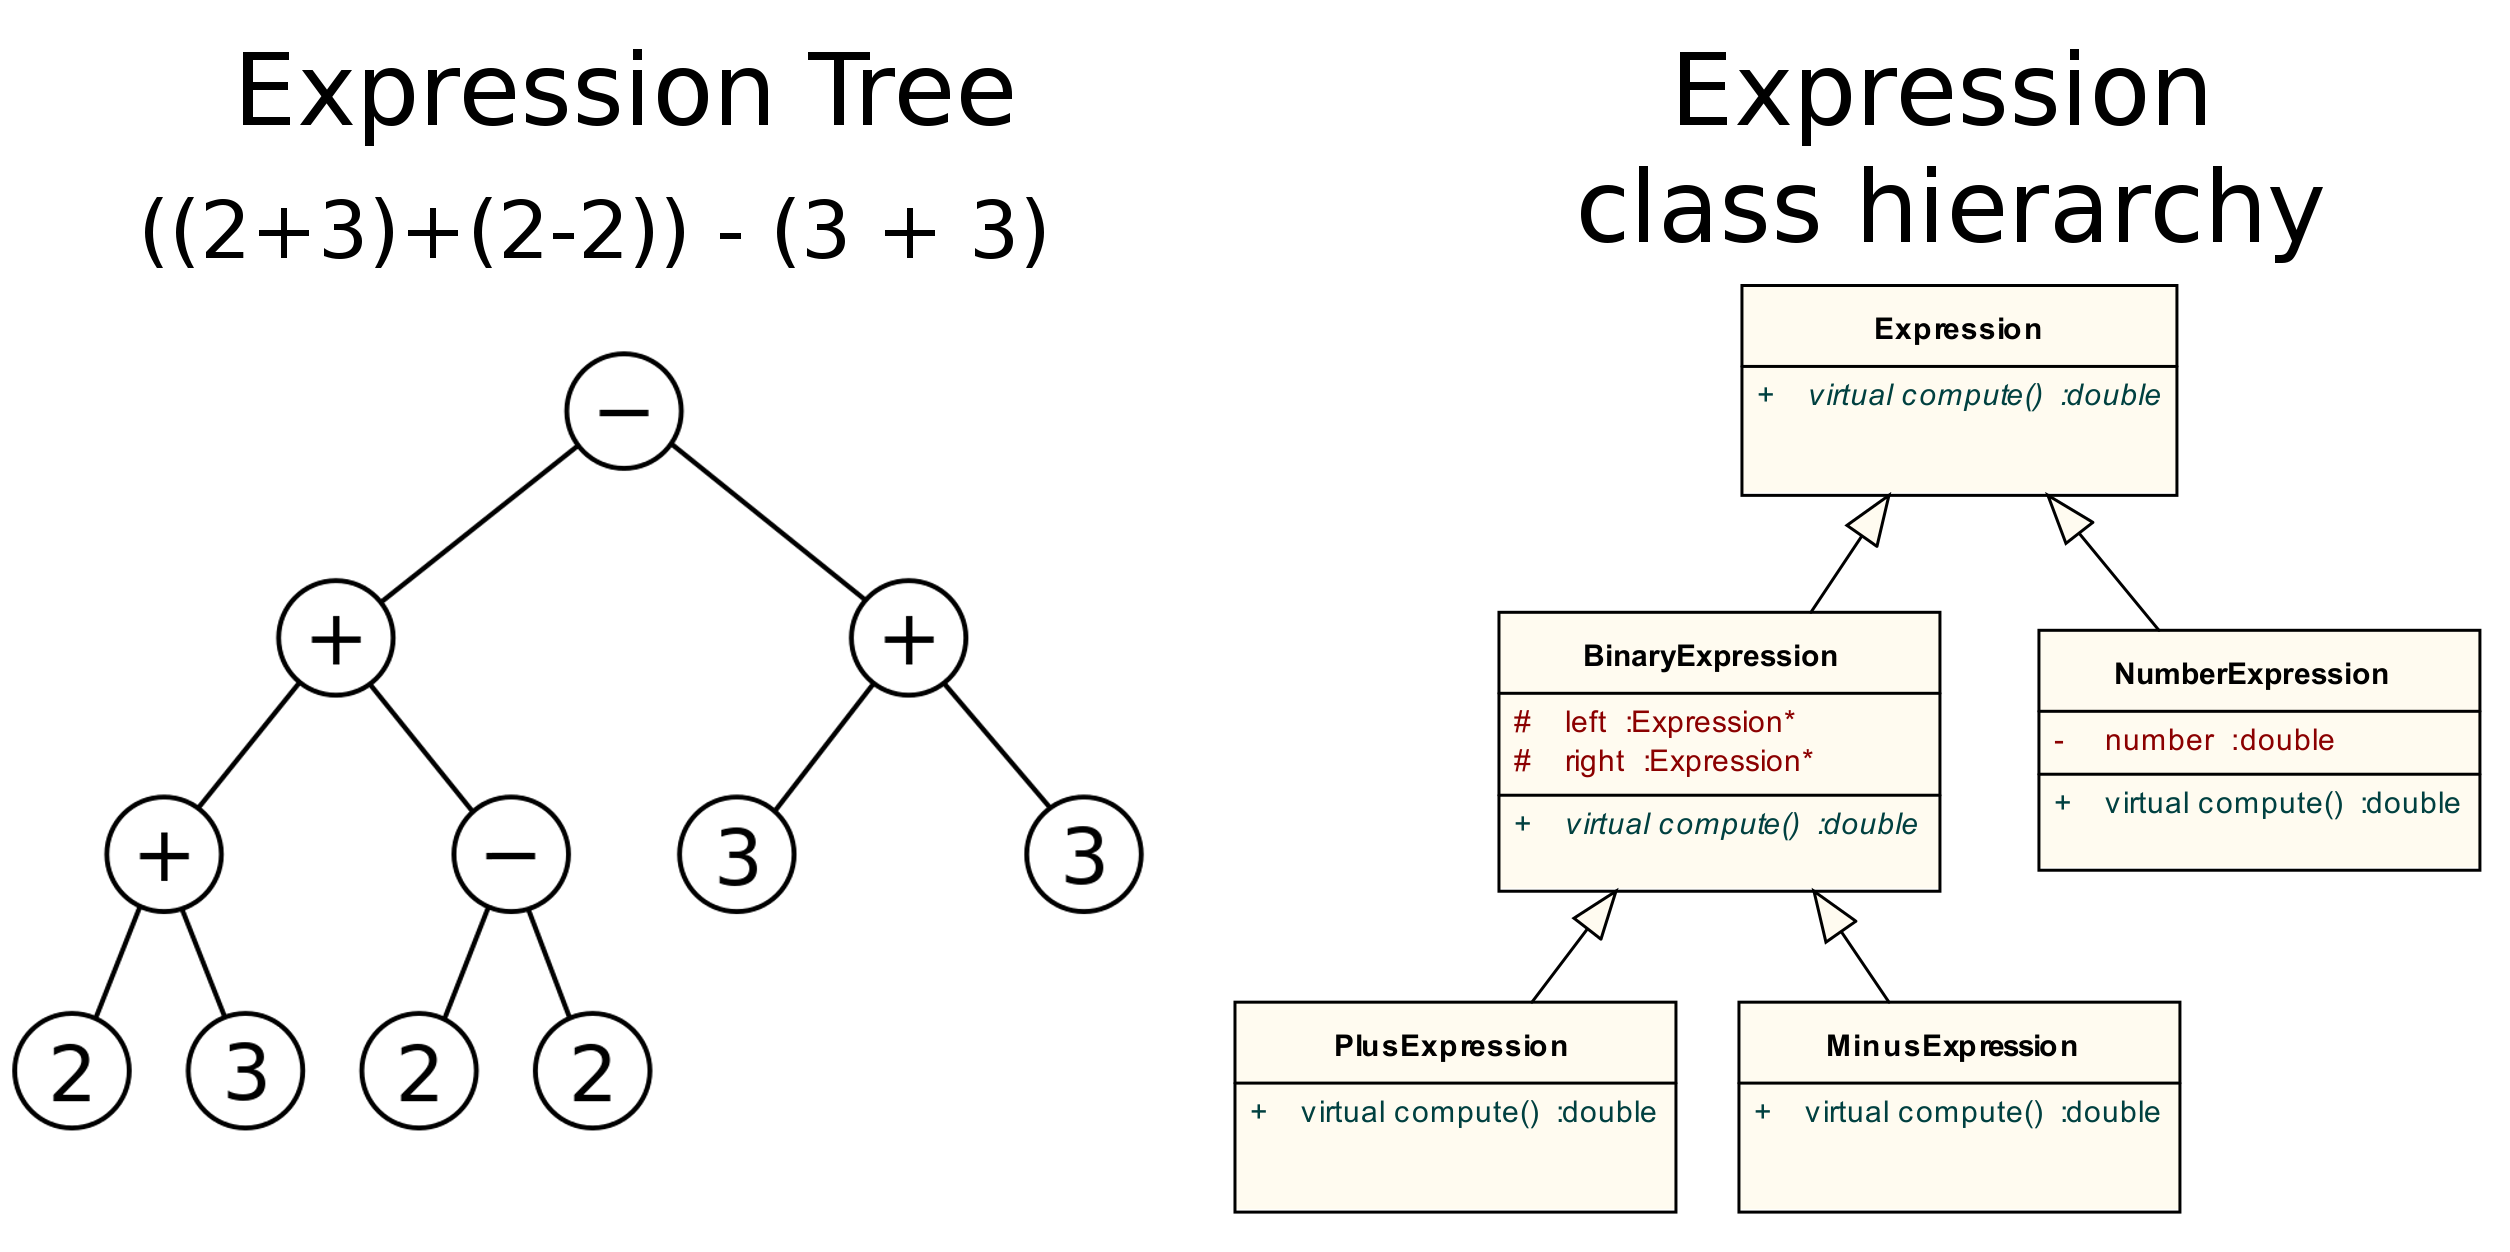
\includegraphics[width=.75\textwidth]{ExpressionTree.png}\\
	Abbildung: Beispielausdruck mit Ausdrucksbaum und Klassenhierarchie.
\end{center}

\begin{enumerate}

\item \textbf{Klasse \emph{Expression}}
Schreibe die abstrakte Klasse \emph{Expression}.
Diese soll als Basisklasse für alle Ausdrücke dienen.
Implementiere einen parameterlosen Konstruktor und einen virtuellen Destruktor, die je eine Meldung auf der Konsole ausgeben, sodass es bei der Ausführung ersichtlich wird, wann eine \emph{Expression} erzeugt und wann zerstört wird.
Deklariere außerdem eine abstrakte (\emph{pure virtual}) Methode \emph{double compute()}, die das Ergebnis des Ausdrucks berechnen und zurückgeben soll. 

\item \textbf{Klasse \emph{NumberExpression}}
Schreibe die Klasse \emph{NumberExpression}, die ein (Baum-)Blatt mit einer Zahl darstellt.
Dementsprechend soll \emph{NumberExpression} von \emph{Expression} erben und ein Attribut zum Speichern einer Zahl besitzen, das im Konstruktor initialisiert wird.
Implementiere den Konstruktor und virtuellen Destruktor und versehe auch diese mit einer Konsolenausgabe.
Die Methode \emph{compute()} gibt die gespeicherte Zahl zurück.

\item \textbf{Klasse \emph{BinaryExpression}}
Schreibe die abstrakte Klasse \emph{BinaryExpression} mit den \emph{protected} Attributen \emph{Expression* left, *right}.
Implementiere den Konstruktor und virtuellen Destruktor mit entsprechender Ausgabe.
Vergiss nicht, im Destruktor die beiden Zweige zu löschen. 

\item \textbf{Klassen \emph{Plus-} und \emph{Minusexpression}}
Schreibe die Klassen \emph{PlusExpression} und \emph{MinusExpression}, die von \emph{BinaryExpression} erben und eine Addition bzw. Subtraktion realisieren. 
Implementiere die Kon- und Destruktoren sowie die \emph{compute()} Methode.

\item \textbf{Test}
Teste deine Implementierung.
Ein gutes Beispiel findest du in Abbildung weiter oben.
Schaue dir die Ausgabe genau an und versuche anhand der gegebenen Klassenhierarchie die Reihenfolge der Erzeugung und Zerstörung von Objekten  nachzuvollziehen.

\end{enumerate}

\section{Fortsetzung Aufzugsimulator}
Unser bisheriger Aufzugsimulator hat eine feste Strategie, nach der die einzelnen Stockwerke abgefahren werden. Mithilfe von Polymorphie können wir den Simulator so erweitern, dass die Strategie austauschbar wird.  

\begin{enumerate}
\item
Lagere die bereits existierende Simulation des Aufzugs aus der \emph{main}-Funktion in eine eigene Funktion \emph{runSimulation()} aus. Die Funktion sollte das volle Gebäude als Parameter entgegennehmen und eine Liste (\emph{std::list<int>}) der angefahrenen Stockwerke zurückgeben. Überlege dir, auf welche Art das Gebäude idealerweise übergeben werden sollte.
Teste deine Implementierung.

\item \textbf{Klasse \emph{ElevatorStrategy}}
Implementiere die Klasse \emph{ElevatorStrategy}.
Diese soll die Basisklasse für verschiedene Aufzugstrategien sein.

\begin{lstlisting}
/**
 * Elevator strategy base class. Determines to which floor the elevator should move next.
 */
class ElevatorStrategy {
public:
	virtual ~ElevatorStrategy();

	/**
	 * Creates a plan for the simulation. 
	 * Default implementation does nothing but saving the building pointer.
	 */
	virtual void createPlan(const Building*);

	/** 
	 * Gets the next floor to visit.
	 */
	virtual int nextFloor() = 0;

protected:
	/** Pointer to current building, set by createPlan() */
	const Building* building;
};
\end{lstlisting}

Damit die Strategie das Gebäude nicht selbst modifizieren kann, wird \emph{Building} per const Pointer übergeben.

\item \textbf{Eine einfache Aufzusstrategie}
Implementiere eine einfache Aufzugstrategie.
Diese soll folgendermaßen vorgehen: 
Falls der Aufzug momentan leer ist, soll zum tiefsten Stockwerk gefahren werden, wo sich noch Personen befinden.
Falls der Aufzug nicht leer ist, wird das Zielstockwerk einer der Personen im Aufzug ausgewählt.

\item \textbf{Implementierung von \emph{runSimulation}}
Ändere nun \emph{runSimulation()} entsprechend um, sodass die Simulation anhand der gegebenen Strategie durchgeführt wird.
Folgender Pseudocode kann dir als Denkhilfe dienen: \\
\begin{algorithm}[H]
 \SetAlgoLined
 \While{People in Building or Elevator}{
   Calculate next floor;\\
   
   Move Elevator to next floor; \\
   Let all arrived people off; \\
   Let all people on floor into Elevator;\\
 }
\end{algorithm}

\item \textbf{Systemtest} 
Teste deine Implementierung mit der bisher erstellten, einfachen Strategie.

\item \textbf{Neue Aufzugstrategien (optional)}
Entwickle eigene Aufzugstrategien. 
Versuche, verschiedene Größen zu optimieren, wie z.B. die Anzahl der Stopps oder die verbrauchte Energie.
Hierfür könnte Backtracking verwenden\footnote{\url{Siehe http://de.wikipedia.org/wiki/Backtracking}}, eine einfache Methode, um optimale Lösungen durch Ausprobieren zu finden. Beachte, dass der Aufzug auch kopiert werden kann, um verschiedene Strategien zu testen.

\end{enumerate}

\end{document}
